\section{Технологический раздел}
\label{sec:technology}

\subsection{Определения стека технологий}

В современной сфере разработки программного обеспечения выбор стека технологий играет ключевую роль в успехе проекта. Стек технологий включает в себя языки программирования, фреймворки, библиотеки и среды разработки, которые совместно обеспечивают качественное создание, тестирование и развертывание приложений. При выборе стека необходимо учитывать множество факторов, таких как целевая платформа, производительность, безопасность, масштабируемость и удобство разработки.

В данном разделе приводится обоснование выбора конкретных технологий и инструментов для разработки программного комплекса организации и выдачи верифицированных цифровых дипломов.

Интегрированная среда разработки (IDE)~\cite{bib:ide_is} или редактор кода являются важнейшими инструментами для программиста. Выбор подходящей платформы может значительно повысить продуктивность и качество кода. Были рассмотрены три популярных решения: WebStorm, Visual Studio Code и NeoVim.

WebStorm~\cite{bib:webstorm}, разработанный JetBrains, является мощной IDE для JavaScript, TypeScript и других смежных технологий. Она предлагает множество встроенных функций, таких как автодополнение кода, отладка, интеграция с системами контроля версий, удаленную разработку и многое другое. WebStorm обеспечивает отличную поддержку для современных фреймворков и библиотек, включая разработку умных контрактов на Solidity. Несмотря на все свои преимущества, WebStorm является ресурсоемким и платным, что делает его менее подходящим для использования.

Visual Studio Code (VS Code)~\cite{bib:vscode}, созданный Microsoft, является одним из самых популярных редакторов кода благодаря своей легковесности и расширяемости. VS Code поддерживает огромное количество плагинов, которые могут добавить функциональность, схожую с полноценной IDE. Он обеспечивает хорошую производительность и поддерживает большинство современных языков программирования и фреймворков, однако, как и WebStorm, VS Code собирает телеметрию и требует значительные системные ресурсы при использовании множества расширений и инструментов.

NeoVim~\cite{bib:neovim} является усовершенствованной версией классического Vim, предлагая более современные возможности и улучшенную расширяемость. Основное преимущество NeoVim заключается в его легковесности, в том числе интерфейса, и возможности создания полностью настраиваемой среды разработки. С помощью различных плагинов и конфигураций, разработчик может собрать идеальную среду для своих нужд, при этом сохраняя высокую производительность даже на слабых компьютерах. NeoVim обеспечивает поддержку автодополнения кода, синтаксического анализа, отладки и интеграции с системами контроля версий, что делает его отличным выбором для разработки программного продукта.

После определния среды для разработки необходимо выделить наиболее подходящии языки программирования и фреймворки для реализации программного комплекса. Требуется выбрать язык для написания умного контракта, программного интерфейса приложения и клиентских приложений для администратора и пользователей системы.

Для разработки сервера и API был выбран Python с библиотекой FastAPI~\cite{bib:fastapi}. Python известен своей простотой и читаемостью, что делает его идеальным для быстрой разработки и прототипирования. FastAPI, в свою очередь, предоставляет высокопроизводительный фреймворк для создания API, который поддерживает асинхронное программирование и автоматически генерирует документацию. Основные преимущества заключаются в следующем:

\begin{itemize}
    \item Простота и читаемость кода.
    \item Быстрая разработка и развертывание.
    \item Поддержка асинхронного программирования.
    \item Автоматическая генерация документации API.
\end{itemize}

В случае с умным контрактом был выбран язык Solidity, который идеально подходит к задаче благодаря своей специализации на EVM (Ethereum Virtual Machine)~\cite{bib:evm}. Этот язык программирования был специально разработан для написания смарт-контрактов на блокчейне Ethereum и других совместимых с ним блокчейнов. Solidity обладает богатым набором функций, позволяющих эффективно работать с контрактами, и имеет широкую поддержку в сообществе разработчиков блокчейн. Его синтаксис основан на JavaScript, что сильно облегчает изучение и разработку. Выбор был сделан на основе нижеприведенных факторов:

\begin{itemize}
    \item Оптимизирован для EVM.
    \item Широкая поддержка блокчейнов.
    \item Большое сообщество и множество доступных ресурсов.
    \item Хорошая интеграция с инструментами разработки и тестирования.
\end{itemize}

Для разработки клиентской части приложения был выбран TypeScript в сочетании с React~\cite{bib:react}. TypeScript является строго типизированным надмножеством JavaScript, что позволяет избежать ряда ошибок на этапе компиляции и улучшает качество кода. React, как один из самых популярных фреймворков для создания пользовательских интерфейсов, обеспечивает высокую производительность и удобство разработки благодаря своей компонентной архитектуре.

Преимущества TypeScript:
\begin{itemize}
    \item Статическая типизация снижает количество ошибок.
    \item Улучшенная поддержка IDE и автодополнение кода.
    \item Совместимость с JavaScript.
\end{itemize}

Преимущества React:
\begin{itemize}
    \item Компонентная архитектура облегчает повторное использование кода.
    \item Высокая производительность и эффективность.
    \item Широкое сообщество и богатый экосистемой библиотек и инструментов.
\end{itemize}

\subsection{Разработка компонентов системы}

При разработке необходимо обращать внимание не только на стек технологий, но и на паттерны проектирования. Сейчас существует множество шаблонов проектирования и подходов, которые помогают создавать эффективные, поддерживаемые и масштабируемые приложения. В этом разделе были рассмотрены некоторые из популярных паттернов.

\subsubsection{Шаблоны проектирования}

Шаблоны проектирования представляют собой проверенные решения для типичных задач, с которыми сталкиваются разработчики. Они помогают структурировать код и улучшить его качество. В данном проекте были использованы следующие шаблоны проектирования:

\begin{enumerate}
    \item \textit{Фабричный метод (Factory Method).}
    \begin{enumerate}
        \item Используется для создания объектов без необходимости указывать точный класс создаваемого объекта.
        \item Применяется в системе для создания различных типов токенов или объектов данных.
    \end{enumerate}
    \item \textit{Одиночка (Singleton).}
    \begin{enumerate}
        \item Обеспечивает наличие единственного экземпляра класса и предоставляет глобальную точку доступа к нему.
        \item Используется для управления подключением к базе данных или другим сервисам, которые должны быть доступны из разных частей приложения.
    \end{enumerate}
    \item \textit{Декоратор (Decorator).}
    \begin{enumerate}
        \item Позволяет динамически добавлять новую функциональность объектам.
        \item Применяется для расширения возможностей базовых компонентов интерфейса без изменения их кода.
    \end{enumerate}
\end{enumerate}

\subsubsection{Подходы к разработке}

Разработка программного обеспечения включает различные подходы, которые помогают организовать процесс и структуру кода. В этом проекте были использованы следующие подходы:

\begin{enumerate}
    \item \textit{DDD (Domain-Driven Design).}
    \begin{enumerate}
        \item DDD фокусируется на модели предметной области и использовании языка, понятного всем участникам проекта.
        \item В проекте используется DDD для создания модели данных и логики бизнес-процессов, что обеспечивает лучшее понимание требований и упрощает поддержание кода.
    \end{enumerate}
    \item \textit{TDD (Test-Driven Development).}
    \begin{enumerate}
        \item TDD предполагает написание тестов перед реализацией функциональности.
        \item Этот подход помогает обеспечить высокое качество кода и уменьшить количество ошибок, возникающих в процессе разработки.
    \end{enumerate}
\end{enumerate}

\subsubsection{Архитектура программного обеспечения}

Архитектура программного обеспечения описывает структуру системы, взаимодействие между компонентами и потоки данных. В этом разделе были рассмотрены архитектуры фронтенда и бэкенда.

Фронтенд системы был реализован с использованием React и TypeScript. Основные элементы архитектуры включают:

\begin{enumerate}
    \item \textit{Компоненты.}
    \begin{enumerate}
        \item Приложение состоит из отдельных компонентов, каждый из которых отвечает за свою часть интерфейса.
        \item Компоненты могут быть повторно использованы или работать независимо.
    \end{enumerate}
    \item \textit{Состояния.}
    \begin{enumerate}
        \item Для управления состоянием приложения используется Context API или Redux.
        \item Это обеспечивает централизованное управление состоянием и упрощает передачу данных между компонентами.
    \end{enumerate}
    \item \textit{Роутеры (маршрутизаторы).}
    \begin{enumerate}
        \item Используется для управления навигацией внутри приложения.
        \item Позволяет создавать одностраничные приложения (SPA) с плавным переходом между страницами.
    \end{enumerate}
\end{enumerate}

Код приложения для администратора приведен в приложении~\ref{appendix:sd_adm_webapp}, а клиентская часть для пользователей в приложении~\ref{appendix:sd_user_telegram}.

Бэкенд системы реализован с использованием Python и FastAPI. Основные компоненты архитектуры включают:

\begin{enumerate}
    \item \textit{REST API.}
    \begin{enumerate}
        \item FastAPI используется для создания RESTful API, который обеспечивает взаимодействие с фронтендом.
        \item API обеспечивает доступ к функциональности системы, такой как создание и управление токенами, получение данных и выполнение бизнес-логики.
    \end{enumerate}
    \item \textit{Слои приложения.}
    \begin{enumerate}
        \item Контроллеры. Обрабатывает входящие HTTP-запросы, вызывает соответствующие сервисы и возвращает ответы.
        \item Сервисы. Содержит бизнес-логику приложения. Взаимодействует с репозиториями и внешними сервисами
        \item Репозитории. Отвечает за доступ к данным, обеспечивает взаимодействие с базой данных и другими хранилищами данных.
    \end{enumerate}
    \item \textit{Web3 обработчик.}
    \begin{enumerate}
        \item Используется подключение к RPC-узлу для взаимодействия с блокчейн-сетью.
        \item Реализованы функции для создания, одобрения и управления смарт-контрактами на основе Solidity.
    \end{enumerate}
\end{enumerate}

\subsection{Графический пользовательский интерфейс}

В данном разделе были рассмотрены два основных пользовательских интерфейсов программного комплекса: веб-приложение для создания коллекции дипломов администратором и телеграм-бот для просмотра и получения дипломов пользователями. Оба компонента обеспечивают удобство использования и доступ к функциональности системы.

\subsubsection{Веб-приложение для создания коллекции дипломов}

В первую очередь было реализовано веб-приложение для управления. Оно позволяет администратору загружать изображения дипломов, вводить метаданные и прочие параметры коллекции. Реализация состоит из основной страницы с несколькими компонентами, обеспечивающими удобный интерфейс.

Основные функции веб-приложения:
\begin{itemize}
    \item Загрузка изображений дипломов.
    \item Ввод метаданных в формате JSON.
    \item Указание названия, описания и автора коллекции.
    \item Настройка количества требуемых подписей для создания NFT.
\end{itemize}

Авторизация реализована при помощи модуля обратного прокси Caddy~\cite{bib:caddy} и требует токен для входа. После авторизации, на главной странице, администратор может загрузить изображения или архив изображений с дипломами, внести метаданные и указать дополнительные параметры для новой коллекции дипломов. Пример интерфейса приведен на изображении~\ref{fig:s3_admin_webapp}, а код в листинге~\ref{lst:admin_webapp} из приложения~\ref{appendix:sd_adm_webapp}.

\begin{figure}[H]
	\centering
	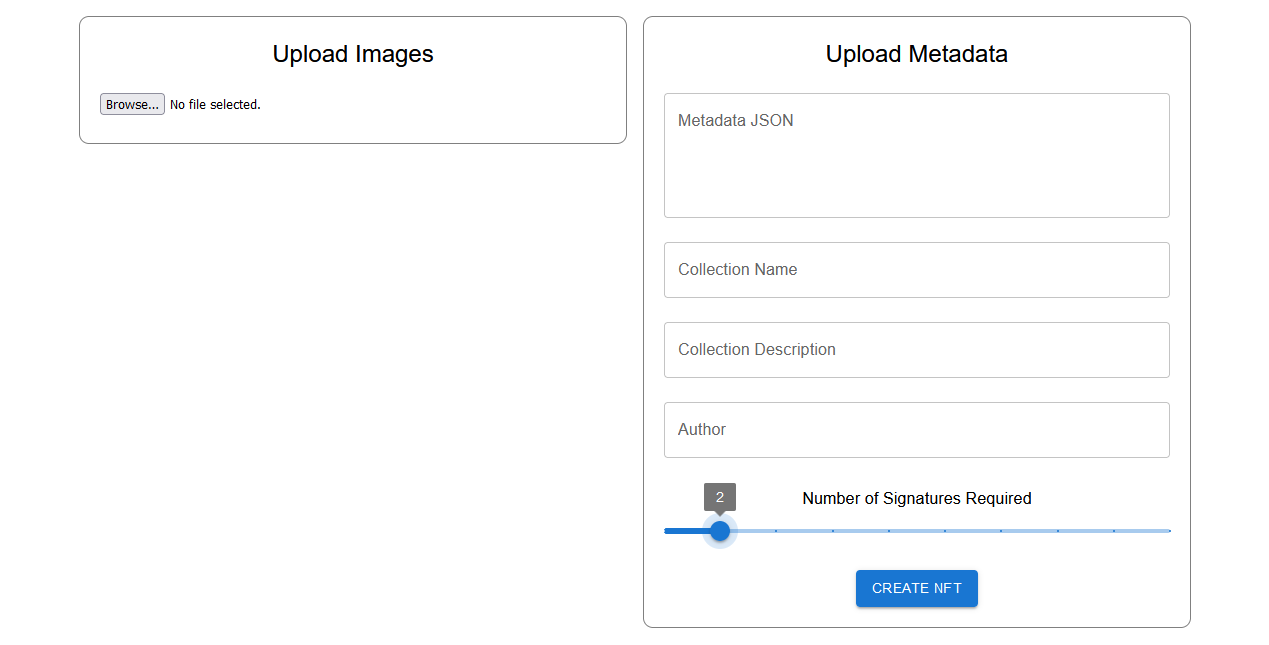
\includegraphics[width=1\textwidth]{images/s3_admin_webapp.png}
	\parskip=6pt
	\caption{Интерфейс администратора для создания коллекции дипломов}
	\label{fig:s3_admin_webapp}
\end{figure}

\subsubsection{Телеграм-бот для просмотра и получения дипломов}

Телеграм-бот был разработан с использованием библиотеки node-telegram-bot-api, код которого приведен в листинге~\ref{lst:user_client} из приложения~\ref{appendix:sd_user_telegram}. Он позволяет пользователям просматривать и получать свои дипломы в формате NFT, обеспечивая удобный интерфейс для взаимодействия с системой через мессенджер. Пример интерфейса приведен на рисунке~\ref{fig:s3_user_client}, где изображено оба окна.

\begin{figure}[H]
	\centering
	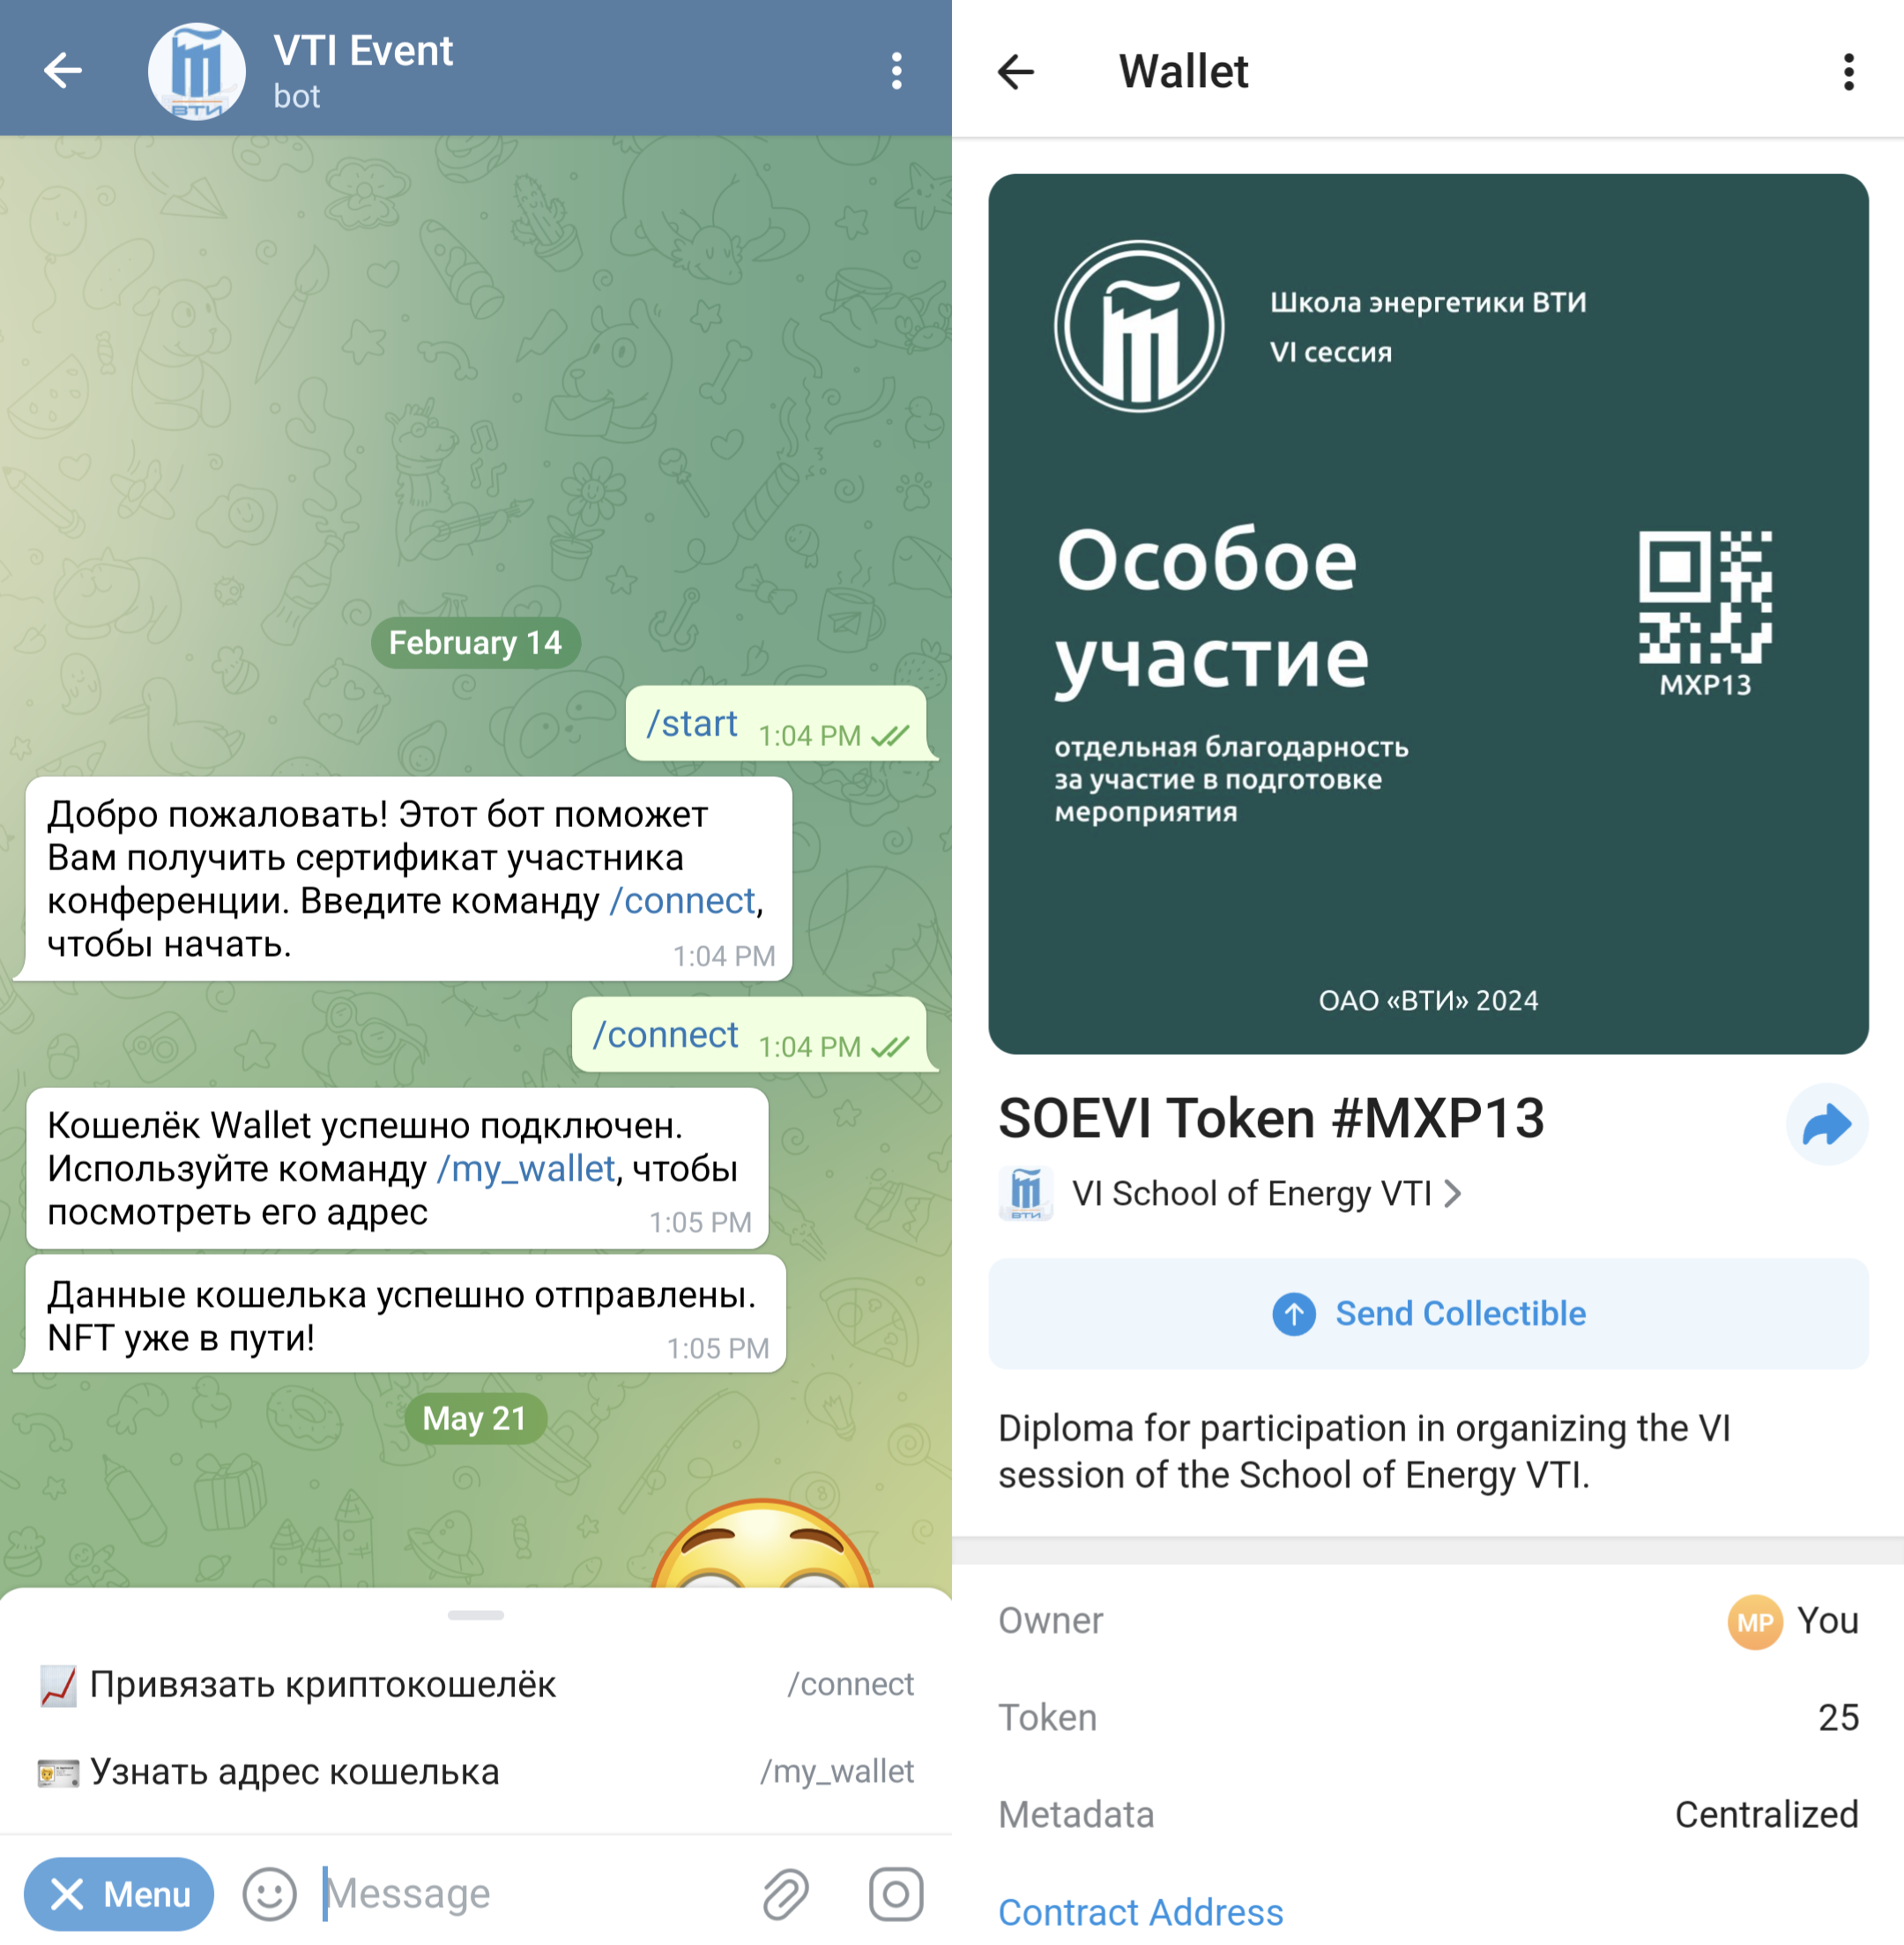
\includegraphics[width=.8\textwidth]{images/s3_user_client.png}
	\parskip=6pt
	\caption{Пользовательский бот для получения и просмотра дипломов}
	\label{fig:s3_user_client}
\end{figure}

Основные функции телеграм-бота:
\begin{itemize}
    \item Просмотр списка доступных дипломов.
    \item Получение информации о конкретном дипломе.
    \item Получение ссылки на NFT-диплом.
\end{itemize}

Пользователи могут взаимодействовать с ботом через простые команды, такие как /start, /connect и т.д. Бот обрабатывает команды, запрашивает данные у API и возвращает пользователям соответствующую информацию.

\subsubsection{Просмотр дипломов на других платформах}

Реализация умного контракта, приведенного в листинге~\ref{lst:smartcon} из приложения~\ref{appendix:sd_smartcon}, для <<ПК Дипломер>> предоставляет значительные преимущества, одной из которых является возможность просмотра данных дипломов на любых платформах, которые умеют взаимодействовать с соответствующей блокчейн-сетью. Это достигается благодаря использованию стандарта ERC-721~\cite{bib:erc721}, широко признанного и поддерживаемого многими блокчейн-платформами и приложениями.

ERC-721 является стандартом для невзаимозаменяемых токенов (NFT) в блокчейне Ethereum и совместимых с EVM (Ethereum Virtual Machine) блокчейнах. Он определяет набор правил бинарного интерфейса приложения (ABI)~\cite{bib:abi_is}, которые должны быть реализованы смарт-контрактами. Это обеспечивает их совместимость с различными децентрализованными приложениями (dApps)~\cite{bib:dapps} и платформами.

Пример прсмотра дипломов на сторонней платформе NFTScan приведен на рисунке~\ref{fig:s3_nftscan}.

\begin{figure}[H]
	\centering
	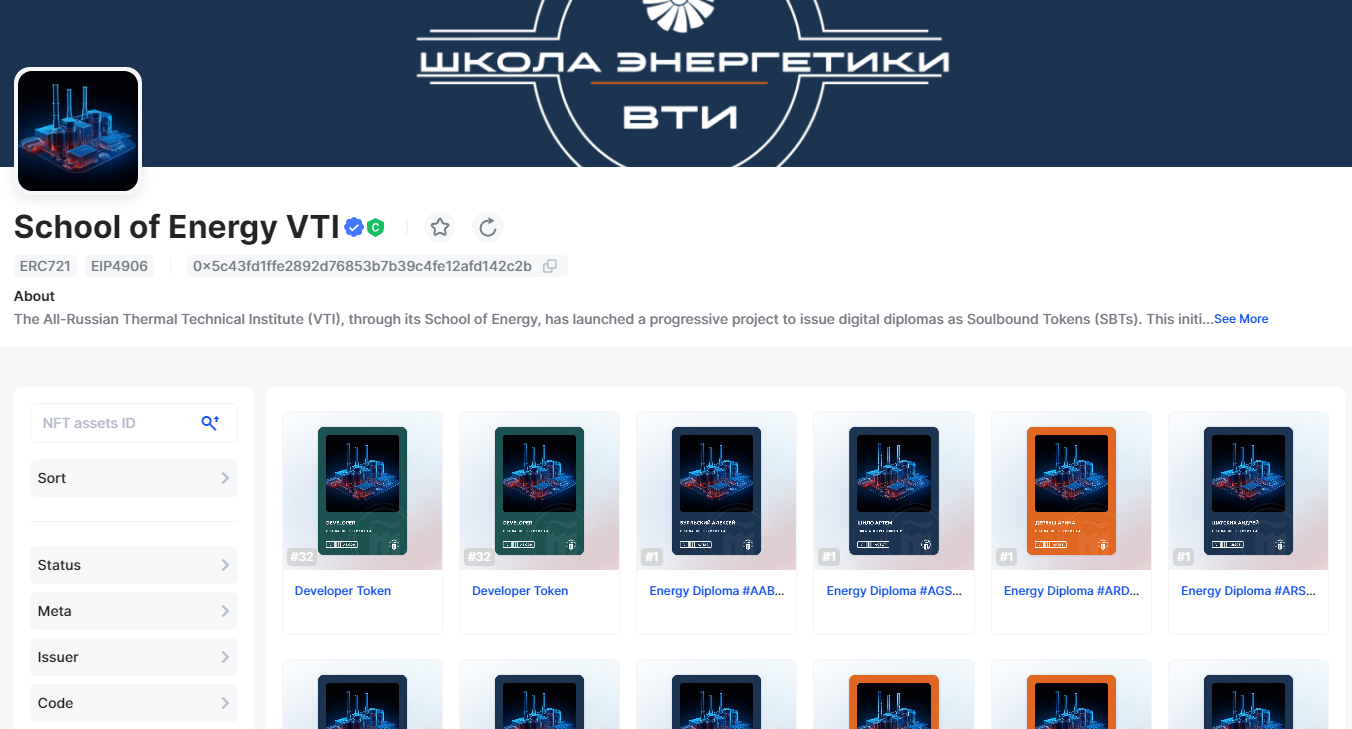
\includegraphics[width=1\textwidth]{images/s3_nftscan.png}
	\parskip=6pt
	\caption{Просмотр дипломов на сторонней платформе}
	\label{fig:s3_nftscan}
\end{figure}

Стоит отметить, что внешние платформы не могут отобразить всю информацию из контрактов, вроде нескольких подписавших, но на отображение самого диплома это не влияет.

\subsection{Серверная часть приложения}

Основная часть системы состоит из двух компонентов: минтера (minter) и API. Эти компоненты обеспечивают взаимодействие клиентских приложений с блокчейном и позволяют пользователям управлять своими дипломами в формате NFT.

\subsubsection{Система выпуска дипломов}

Минтер (minter) является основным компонентом системы, отвечающим за создание новых NFT-документов. Он реализует функциональность выпуска дипломов и взаимодействия с умным контрактом на блокчейне, обеспечивая выполнение всех операций, связанных с созданием и управлением токенами.

Сама функция выпуска диплома лаконичная и отвечает лишь за передачу подготовленных ранее данных в блокчейн. В ней указывается комиссия за транзакцию (газ) и дополнительные пользовательские данные. Код функции приведен в листинге~\ref{lst:minter}.

\begin{lstlisting}[label=lst:minter, language=Python, caption=Функция выпуска диплома]
    def mint(to, uri):
        gas_price = w3.eth.gas_price
        nonce = get_nonce()
        tx = contract.functions.proposeMint(to, uri).build_transaction({
            'chainId': chain_id,
            'gas': 200000,
            'gasPrice': gas_price,
            'nonce': nonce,
        })
        signed_tx = account.sign_transaction(tx)
        tx_hash = w3.eth.send_raw_transaction(signed_tx.rawTransaction)
        receipt = w3.eth.wait_for_transaction_receipt(tx_hash.hex())
        return receipt
\end{lstlisting}

\subsubsection{Программный интерфейс прилоения}

API обеспечивает интерфейс для взаимодействия клиентских приложений с системой. Оно реализовано с использованием FastAPI и предоставляет RESTful сервисы для выполнения различных операций, таких как создание, одобрение и сжигание токенов, а также получение информации о пользователях и токенах.

\begin{itemize}
    \item Создание новых токенов. API предоставляет конечные точки для создания новых токенов, что позволяет клиентским приложениям инициировать процесс создания дипломов.
    \item Одобрение транзакций. Конечные точки для одобрения транзакций обеспечивают возможность мультиподписи.
    \item Получение информации. API позволяет получать информацию о пользователях и токенах, обеспечивая необходимую функциональность для клиентских приложений.
    \item Сжигание токенов. Конечные точки для сжигания токенов позволяют управлять жизненным циклом дипломов.
\end{itemize}

Все существующие в системе маршруты до конечных точек (эндпоинтов) представлены в таблице~\ref{tab:api_routes}.

\begin{table}[H]
	\caption{Маршруты API}
	\centering
	
	\tolerance=0
	\emergencystretch=10pt
	\hyphenpenalty=0
	\exhyphenpenalty=0
	\begin{tabular}{x{3cm}x{3cm}x{7cm}}
		\toprule
		\textbf{Маршрут} & \textbf{Метод HTTP} & \textbf{Описание} \\ \midrule
		/mint & POST & Создание нового NFT-документа \\
		/approve\_mint & POST & Одобрение создания нового NFT-документа \\
		/burn & POST & Сжигание существующего NFT-документа \\
		/balance & GET & Получение баланса (количество NFT) для указанного адреса \\
		/total\_supply & GET & Получение общего количества выпущенных NFT \\
		/roles/add\_minter& POST & Назначение роли MINTER для указанного адреса \\
        /roles/remove\_minter & POST & Удаление роли MINTER у указанного адреса \\
        /roles/add\_multisig & POST & Назначение роли MULTISIG для указанного \\
        /roles/remove\_multisig & POST & Назначение роли MULTISIG для указанного адреса \\ \bottomrule
	\end{tabular}
	
	\label{tab:api_routes}
\end{table}
